\chapter{Specification}
%The techniques that underlie the implementation are formally specified. The requirements of the implementation are given.
In this chapter, the goals of this work and 6 concrete objectives that should be fulfilled for this work to be considered successful are specified.
The chapter goes on to present the limitations of this work and outlines precisely what parts of the training planning process will be covered.
Some further restrictions of the scope of the thesis are made and the accompanying assumptions stated.
Lastly, some restrictions imposed by the data set, both qualitative and ethical, are highlighted.


\section{Aim}
% Description of where our model fits into the workflow of training plans.
\label{sec:aim}

This study aims to create a model that can create detailed weekly training plans for swimmers in the likeness of a specific professional swimming coach.
For this task, the model should utilize historical plans from the coach, a specification of the training week to plan, and information about the athlete for which the plan is made.
The specification for the week includes information about the number of training sessions to be performed, distribution of training load over the intensity zones, the number of sessions for each particular area of focus, and the time left of the macrocycle.
The athlete information includes the athlete's age, gender and specialty. 
\Cref{fig:model_goal} illustrates a possible input and an example output for the finished model.

To be able to compare different models and human coaches we can define a set of objectives that define when two training plans are similar.
These objectives used in this work are
\begin{enumerate}
    \item \label{constraint:tl_total}Training plans are more similar if their total training loads are close.
    \item \label{constraint:tl_zones}Training plans are more similar if their distribution of training load over the intensity zones match.
    \item \label{constraint:tl_week}Training plans are more similar if their distribution of training load over the sessions match.
    \item \label{constraint:order}Training plans are more similar if they contain similar orderings of session types.
    \item \label{constraint:types}Training plans are more similar if they have the same number of sessions of each session type.
    \item \label{constraint:specialty}Training plans are more similar if they have the same number of sessions suited for each competition type (specialty).
\end{enumerate}

\begin{figure}
    \centering
    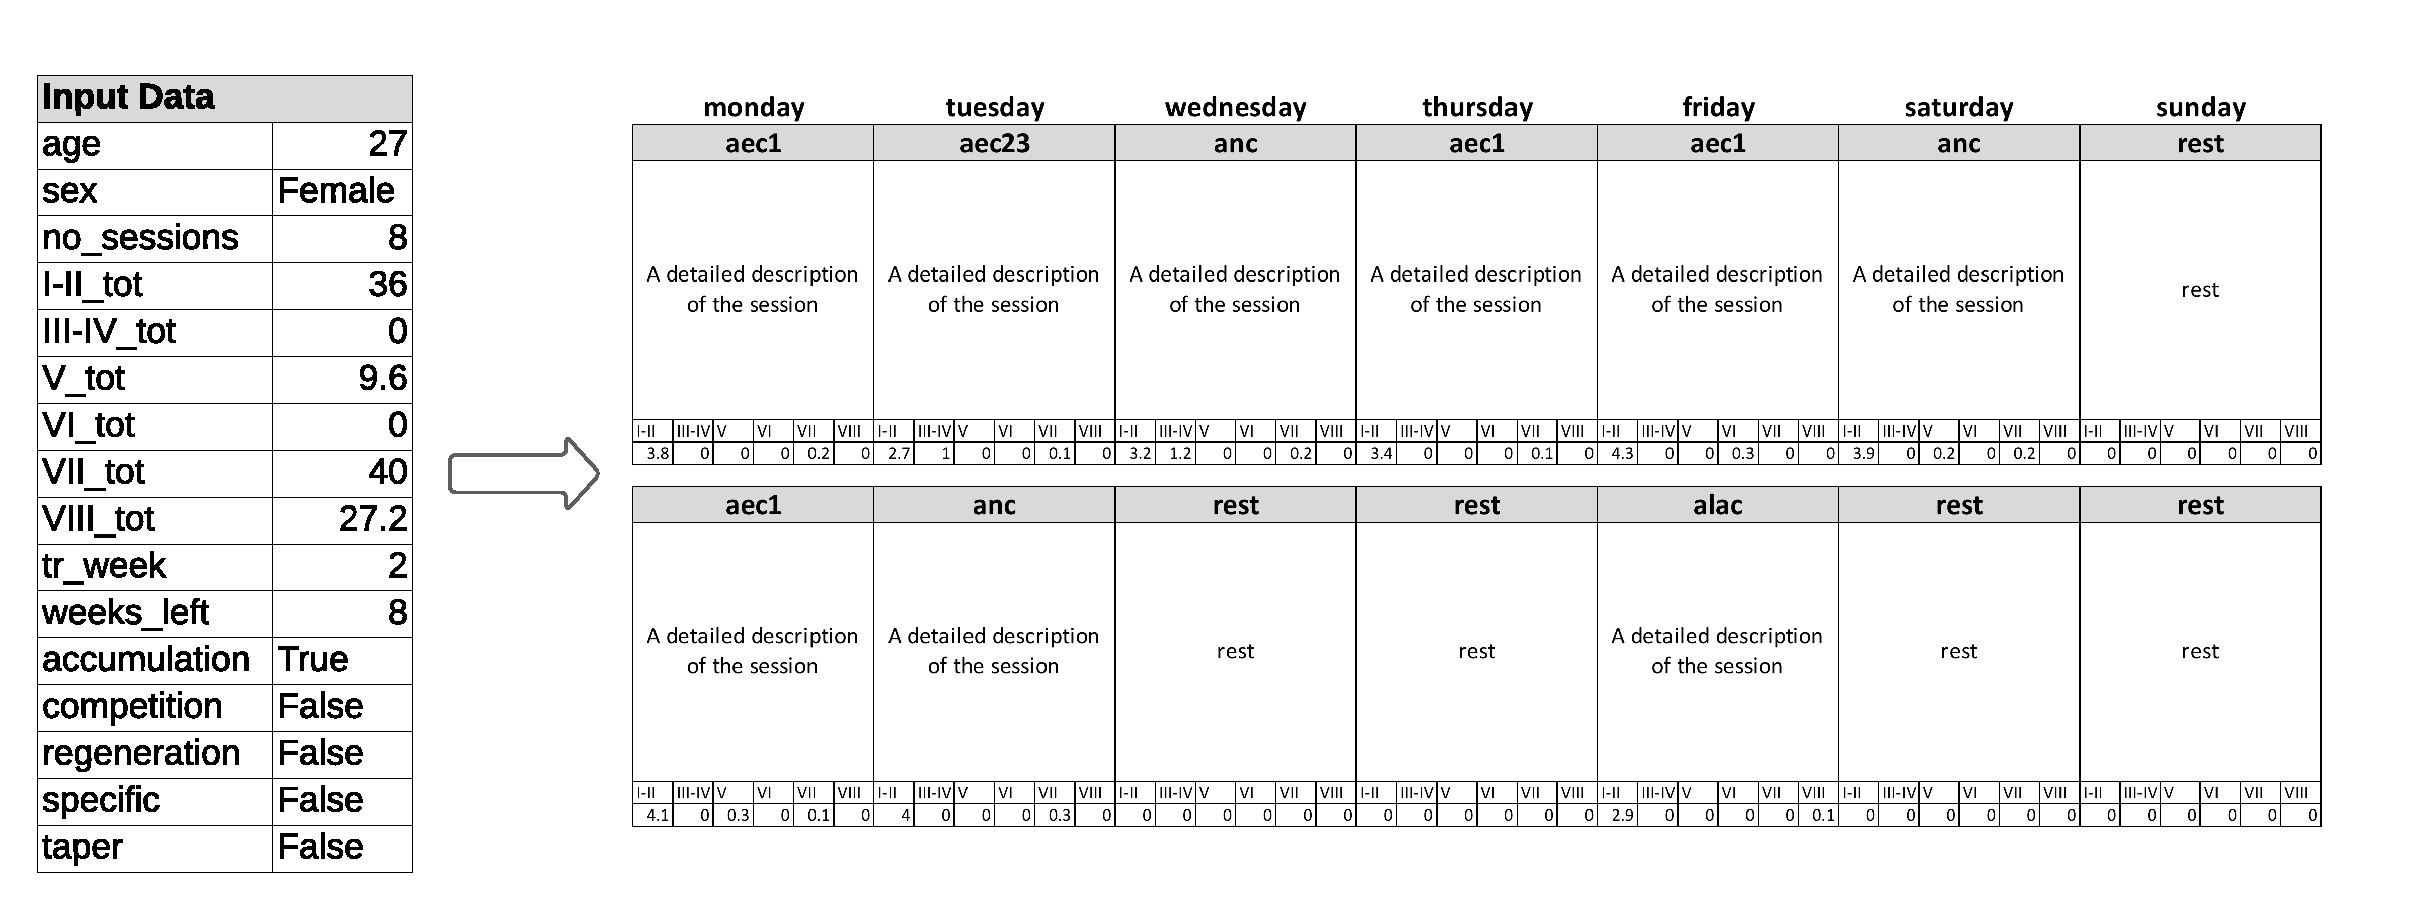
\includegraphics[width=0.9\textheight,angle=90]{chapters/figures/model_goal.pdf}
    \caption{An illustration of the model goals. Weekly information is specified to the left. Based on this information, a weekly training plan similar to the specified coach is generated.}
    \label{fig:model_goal}
\end{figure}

%The aim is a brief description of the assignment and its intended outcome.
% Consider an athlete $A$, recommended training load $L$ for a week, and a detailed training plan $Y$ for the same week.
% Assume that 
% \begin{equation}
%     Y:=f(A,L) \,,
% \end{equation}
% where $f$ is some function describing a specific coach's decision.

% The study aims to develop a method for finding an approximation $\hat{f}$ of $f$.
% For $\hat{f}$ to be considered a valid approximation it should be able to be used to generalize the coach's decision to other athletes and workloads.
% That is, it needs to be possible to substitute $L$ and $A$ with some other $L'$ and $A'$ while keeping $\hat{f}$ fixed to generate a new $\hat{Y}'$ that is close enough to $Y':=f(A',L')$ for the coach to consider it a good match.
% This goal can be reduced down to several research questions.

% \begin{itemize}
%     \item \textit{Is it possible to identify a coach's style based on observed data?}
%     \item \textit{Can identified styles be generalized to other athletes?}
%     \item \textit{How do we measure the "similarity" between our output and a coach's actual training regimen?}
% \end{itemize}



\section{Limitations}
\label{sec:limitations}
%This chapter describes what issues will not be dealt with in the work.
The complete process of training planning consists of multiple subtasks addressing small parts of the problem at multiple scales.
First, the macro and meso plans need to be created. 
This involves scheduling around where important competitions lie and structure training to achieve peak performance at those competitions.
This task will not be addressed in this study, but it is assumed to already be done and that the model has access to some of the information from that plan, such as time left to when peak performance should be achieved and the main focus for each week.
It is also assumed that each week of training is independent.
Although the type of training one week is dependent on what has been done the previous weeks, it is assumed that this has already been accounted for in the macro and meso planning stages.

Secondly, the overall training load needs to be optimized to achieve the appropriate physical response from the athlete.
This is also out of scope for this study and assumed to have been completed beforehand so that the model can rely on the weekly training load being properly adapted for the athlete. 
Furthermore, the physical response of the athlete could be analysed and the performance for some given future training modeled, but this is not explicitly investigated in this study.
Some basic athlete parameters (age, sex, specialty) will however be utilized by the model, together with historical training data on what the coach previously prescribed to the athletes.
If the athlete parameters influence what training the coach prescribes to which athlete then the machine learning part of the model might identify that pattern and possibly mimic it, but no explicit athlete response modeling will be performed in this study.

Lastly, when a weekly detailed plan is executed by the athlete, other factors, such as sleep, diet and stress, might influence the athlete's daily form.
Based on this, the detailed plan could be adjusted to better fit the current circumstances.
How to handle this feedback loop will not be investigated in this study.

To limit the scope of the thesis, the following assumptions are made.
Firstly, it is assumed that the training that the athletes performed is the same that the coach planned.
This assumption is necessary since the training plans themselves are not reliably recorded.
It will, however, make it impossible for the model to disregard changes made to the plan based on daily form.
Since the factors influencing this change have not been recorded, any such changes will most likely appear as noise to the model.

Secondly, we restrict the solution space to have 14 sessions per week and two sessions per day, one before noon one after. 
Further, in this study, we only consider swim training.
Dryland or gym training will not be included.

There are also limitations regarding the data that is used in this study.
Firstly, all data is from elite athletes, all with the same coach.
This makes it impossible to thoroughly test, using this data, if the model developed generalizes to other coaches or other levels of athletes.

Secondly, during this study, we are working with personal information and confidential data.
This has to be carefully considered since a breach can cause irremediable damage to all parties sharing and handling the data.
Neither the data set nor the trained model from this study will be made publicly available.
Only a small, manually curated and controlled, set of direct model outputs will be available together with safe performance metrics and statistics of the model.
This should prevent any breaches from occurring.





% Description of what is not included.

% Things such as generating athlete representation or macro information.
% Assumptions made of what is given to us.
% No difference between planned training and performed training.
% Confidential data / personal information

% {\color{red}For a model to be able to produce output that is individualized for the athlete the input must contain a representation of that athlete.
% Each athlete in our data set has parameters associated with them derived from a model similar to the one in \cite{mujika1996modeled}. The parameters represent physical attributes such as response to training and recovery time needed.

% This study will not go into detail on how this representation is created nor investigate possible alterations.
% Since the representation has been shown to adequately represent athletes from a ``training response''-point of view, we are confident that it is a working representation for our use case as well.}

% To start with, the study will be limited to the sport of swimming and also to a specific coach. In a later stage, it might be possible to lift one or both of these restrictions to investigate the method's ability to generalize.

% Finally, we are working with personal information and confidential data. We have to make sure that the model does not compromise the integrity of the data. This means that we have to train and test the models in a way that makes sure that no information about the training data can be extracted from the model by specially tailored input as an example.

